\documentclass[a4paper,12pt]{article}
\usepackage{fancyhdr}
\usepackage[hmargin=1.75cm,vmargin=1.75cm]{geometry}
\usepackage{graphicx}
\usepackage{amsfonts}
\usepackage{amsmath}
\usepackage{hyperref}
\usepackage{breakurl}
\usepackage[numbers]{natbib}
\usepackage{url}
\usepackage{subfigure}
\usepackage{booktabs}
\bibliographystyle{unsrtnat}
\title{Caspian}
\author{Andrew Clegg\\\href{mailto:andy2.0@gmail.com}{andy2.0@gmail.com}}

\begin{document}
\maketitle
\abstract{\textit{
Caspian is a spatial data gridder operating on binary files containing latitudes, longitudes and observations. Caspian can project these observations onto a grid, reducing data using an appropriate algorithm.
}}
\tableofcontents
\section{Overview}
Gridding is the process of placing observed spatial data (from satellites, planes, or \textit{in-situ} sensors) onto a regular spatial grid. This are many methods to achieving this with different advantages and disadvantages; these include warping an image by comparing known control points, formulating a grid originating from the satellite or plane, and treating each point as an individual observation and placing these observations onto the grid individually. Data reduction is a key aspect of this process, as multiple observations often end up aligned to a single grid point.

Caspian is a gridder that treats data as a mass of individual observations, and grids this data using a variety of data reduction algorithms. Data is projected into the desired projection and loaded into an index, which takes the form of an adaptive K-D tree; a grid is formed and divided into cells, and each of these cells is filled by querying the index for points that fall into the cell, and then using a data reduction algorithm to derive a single value for that cell.

\section{Input and Output Formats}
Both inputs and outputs are in the form of flat binary files. Latitudes and longitudes are input and output in 32-bit IEEE float; the format of the data file (input and output) is specified at run time.

There are 2 modes that decide how the data is interpreted, and what mapping functions can be used. These modes are numeric, and coded. Coded mode is for data that cannot be handled as a number (numeric); some sort of binary data (such as flags) stored in a grid. When handling data of this type, the size of each item of data is specified (\textit{coded8}, \textit{coded16}, \textit{coded32}...), and the contents of the data are never modified.

\section{Specifying the output grid}
A variety of parameters are needed to specify the output grid.
\begin{description}
\item[Projection Description (\texttt{--projection})] This is a PROJ.4 projection specifier string. See \url{http://www.remotesensing.org/geotiff/proj_list/} for a list of common projections, and how to specify them using a PROJ.4 string.
\item[Grid Centre (\texttt{--central-x}, \texttt{--central-y})] -- the offset from the projection origin (units of metres), at which the centre of the output grid will be located.
\item[Horizontal \& Vertical Resolution (\texttt{--hres}, \texttt{--vres})] specify the resolution of the output grid (units of metres).
\item[Width \& Height (\texttt{--width}, \texttt{--height})] specify the width and height of the output grid, in pixels.
\end{description}

As an example, imagine a grid centered over the United Kingdom, using a Mercator projection and the WGS84 datum. The bounds of latitude are (47, 63), and of longitude are (-15, 13). It is designed that the latitude of true scale shall be 55.0. The basic PROJ.4 string for this is ``\texttt{+proj=merc +ellps=WGS84 +lat\_ts=55.0 +lon\_0=-15.0}". Horizontal and vertical resolution are arbitrarily set to 1100 metres.

The central grid position and width and height now need to be computed. For convenience, a utility is provided to do this (built under bin/projcalc).
\begin{verbatim}
bin/projcalc "+proj=merc +ellps=WGS84 +lat_ts=55.0 +lon_0=-15.0" \
   63.0 47 -15 13 1100 1100
Centre: (895917.812500, 4303742.500000)
Width: 1629, Height: 1647
\end{verbatim}
This command has provided the remaining parameters. Note that this command is not applicable in all cases (such as polar stereographic projections); this is why the bounding latitudes and longitudes are not provided directly to Caspian.

\section{Controlling mapping}
The main controls over mapping are in the selection of the mapping function, and in the selection of the sampling rates.
\begin{figure}
\centering
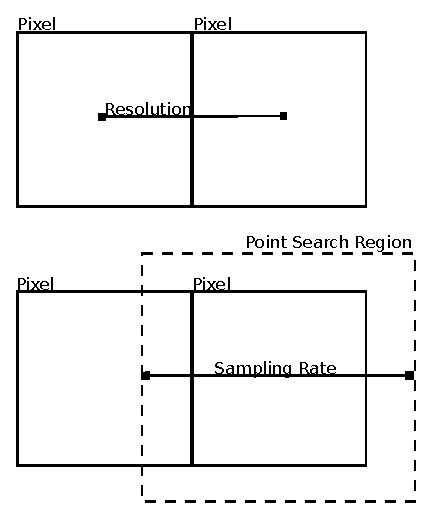
\includegraphics{resolution_and_sampling.eps}
\caption{Diagram showing the difference between resolution and sampling rate}
\label{fig:res_and_sampling}
\end{figure}
\subsection{Sampling Rate}
While the horizontal and vertical resolution define the distance between pixel centres, the sampling rate defines the size of the search box which is used to gather data for that pixel (see Figure~\ref{fig:res_and_sampling}). The simplest case is when the sampling rate is equal to the resolution; in this case the box is equal to the pixel itself. However, to avoid gaps in the output image, it may be necessary to expand the search box outside the bounds of the pixel, in which case the sampling rate may be increased.

To set the sampling rate, use \texttt{--vsample} and \texttt{--hsample}. By default these are equal to the vertical and horizontal resolutions respectively.

\subsection{Mapping Function}
There are currently five mapping functions; four of which can be used with numerical data and one of which can be used for coded data.
\begin{description}
\item[Mean] -- a simple mean of all selected points.
\item[Weighted Mean] -- a mean of all selected points, weighted by distance. The distance is the euclidean distance between the selected point and the centre of the pixel (in metres).
\item[Median] -- the value of the pixel is the median value of all selected points, regardless of their distance from the centre of the pixel.
\item[Newest] -- uses additional per-pixel time information to select the newest pixel found in a given cell.
\item[Nearest Neighbour (Coded)] -- the value of the pixel is the value of the nearest point to the centre.
\end{description}


\section{Usage}

Once the projection parameters have been calculated, and the input data is assembled, usage is simple. For this example, the same projection as before has been used, and the data is assumed to be in float32 format. Sampling rates are set to 3x the resolution.
\begin{verbatim}
bin/caspian --input-data data --input-lats latitudes \
--input-lons longitudes --output-data uk_data \
--output-lats uk_lats --output-lons uk_lons \
--projection "+proj=merc +ellps=WGS84 +lat_ts=55.0 +lon_0=-15.0" \
--width 1629 --height 1647 --hres 1100.0 --vres 1100.0 \
--central-x 895917.8125 --central-y 4303742.5 \
--input-dtype float32 --output-dtype float32 \
--hsample 3300.0 --vsample 3300.0
--mapping-function median
\end{verbatim}

The output files (uk\_data, uk\_lats, and uk\_lons) will all have the same size (equal to width*height); the uk\_lats and uk\_lons files specify geolocation for the projected data.

\subsection{Re-using the spatial index}
Caspian performs two main tasks; generating a spatial index to use for gridding, and then performing the actual gridding. A spatial index takes into account latitude, longitude (and potentially time) information for each pixel, and is specific to a given projection. However, it is not tied to a particular set of data values. Because of this, when gridding different products generated from the same set of data, it is possible to speed up the overall process by generating a spatial index once and using it for all further gridding tasks.

To generate an index to save to disk, you must provide values for \texttt{--input-lats}, \texttt{--input-lons}, \texttt{--projection}, \texttt{--save-index}, and optionally \texttt{--input-time}. The index will then be generated, and saved to the file specified by \texttt{--save-index}.

To load and use the index, run Caspian again, this time providing \texttt{--load-index} with the index filename, and leaving out the latitude, longitude and time filenames and the projection string. Caspian will load the index from disk and from there behave as normal.

\end{document}
